\documentclass[12pt,a4paper]{article}

% ── Packages ──────────────────────────────────────────────────────────────────
\usepackage[T1]{fontenc}
\usepackage[utf8]{inputenc}
\usepackage[margin=2.5cm, headheight=15pt]{geometry}
\usepackage{amsmath,amssymb}
\usepackage{graphicx}
\usepackage{booktabs}
\usepackage{array}
\usepackage{xcolor}
\usepackage{hyperref}
\usepackage{caption}
\usepackage{subcaption}
\usepackage{enumitem}
\usepackage{parskip}
\usepackage{titlesec}
\usepackage{fancyhdr}
\usepackage{microtype}
\usepackage{listings}
\usepackage{float}
\usepackage{tikz}
\usetikzlibrary{shapes.geometric, shapes.misc, arrows.meta, positioning, fit, backgrounds, calc}

\hypersetup{
  colorlinks=true, linkcolor=blue!70!black,
  citecolor=blue!70!black, urlcolor=blue!70!black
}

\pagestyle{fancy}
\fancyhf{}
\rhead{\small Agentic Self-Correction in LLaMA3 --- E-Commerce Sentiment Analysis}
\lhead{\small PES MTech Project}
\rfoot{\small Page \thepage}

% ── Title ─────────────────────────────────────────────────────────────────────
\title{
  \textbf{Agentic Self-Correction in LLaMA3:}\\
  \textbf{Enhancing E-Commerce Sentiment Analysis}\\
  \textbf{through Multi-Agent Reflection}\\[0.5em]
  \large Baseline (Phase~1) + Proposed Agentic Framework (Phase~2)\\[0.3em]
  \normalsize Experimental Results on Amazon Reviews 2023 --- 2\,000 Samples
}
\author{PES MTech Project\\[0.3em]
  \small \texttt{github.com/kvarun314/pes-mtech-project}
}
\date{March 2026}

\begin{document}
\maketitle
\tableofcontents
\newpage

% ══════════════════════════════════════════════════════════════════════════════
\section{Abstract}
% ══════════════════════════════════════════════════════════════════════════════

Automated Sentiment Analysis (ASA) plays a critical role in modern e-commerce systems by
enabling businesses to analyse large volumes of customer feedback and identify trends related
to product quality and user satisfaction. Recent advances in Large Language Models (LLMs),
particularly LLaMA-3, have significantly improved sentiment classification due to their strong
contextual understanding and language reasoning capabilities.

However, these models typically operate as static, text-only classifiers: they generate
predictions in a single inference step without performing factual verification or reflective
reasoning. This leads to \emph{sentiment hallucinations} (e.g.\ incorrectly treating a user's wrong
claim as a real product defect), \emph{context blindness} (missing image and metadata signals),
and \emph{linguistic errors} on sarcasm or mixed-sentiment phrasing.

This paper proposes a multimodal \textbf{Agentic AI framework} for sentiment analysis that
integrates review text, product images, and product metadata to improve classification
reliability. A four-agent pipeline --- Analyst, Visual Verifier, RAG Prover, Critic --- with a
dissonance-triggered self-correction loop is evaluated on 2\,000 samples from the Amazon
Reviews 2023 dataset (All Beauty category).

\medskip
\noindent\textbf{Key results (Run~1):}
\begin{center}
\begin{tabular}{lrrr}
\toprule
\textbf{Metric} & \textbf{Phase~1} & \textbf{Phase~2} & \textbf{$\Delta$} \\
\midrule
Accuracy    & 0.1610 & 0.3870 & +22.60~pp \\
Macro F1    & 0.0946 & 0.2725 & +17.79~pp \\
MAE         & 1.5205 & 0.9635 & $-$0.557 \\
\bottomrule
\end{tabular}
\end{center}

% ══════════════════════════════════════════════════════════════════════════════
\section{Problem Statement}
% ══════════════════════════════════════════════════════════════════════════════

Current AI models used for sentiment analysis excel at language understanding but struggle
with factual accuracy. Because models like LLaMA-3 process a review in a single
``text-only'' step, they lack the ability to verify whether a customer's claims are true. This
produces three primary failure modes:

\begin{enumerate}[leftmargin=*]
  \item \textbf{Sentiment hallucinations.} The AI mistakes a user's incorrect claim (e.g.\
    ``this watch isn't waterproof'') for a legitimate product defect, even if the product
    specification proves otherwise. The model has no access to spec sheets.

  \item \textbf{Context blindness.} By ignoring product images and technical metadata, the AI
    misses vital evidence that could confirm or refute a complaint. A user might write a
    neutral review but upload a photo of a shattered screen; a text-only system is blind to
    this visual evidence.

  \item \textbf{Linguistic errors.} Without a double-check mechanism, models frequently
    misinterpret sarcasm or mixed feelings. ``Amazing, it broke in two days'' may be scored
    positively if the model focuses on ``amazing'' and there is no critic to trigger
    re-evaluation.
\end{enumerate}

\noindent\textbf{The gap:} A system is needed that does not just \emph{read} sentiment but
\emph{verifies} it against product facts and other modalities.

% ══════════════════════════════════════════════════════════════════════════════
\section{Research Gap}
% ══════════════════════════════════════════════════════════════════════════════

\subsection{Baseline Study: Supervised Fine-Tuning with LLaMA-3 (Wang et al., 2025)}

The baseline establishes a benchmark for sentiment classification using LLMs.
\textbf{Model:} LLaMA-3-8B with Low-Rank Adaptation (LoRA) --- only low-rank matrices $A$
and $B$ are updated while primary weights are frozen.
\textbf{Data strategy:} (1) DQC (Data Quality Control) via TextBlob to filter noisy reviews;
(2) VGST (Variant Greedy Search) for diversity-maximising sampling.
\textbf{Reasoning:} One-Shot Learning combined with Zero-Shot CoT prompts.

Paper-reported performance: Accuracy 92.6\%, Precision 95.3\%, F1 93.3\%, outperforming
SVM and XLNet.

Our Phase~1 implementation uses LLaMA-3-8B + PEFT/LoRA ($r$=16, $\alpha$=128, 5 epochs,
\texttt{max\_samples}=4000) with typical Colab eval around $\sim$66\% accuracy and $\sim$68\%
weighted F1. Despite strong paper numbers, the baseline is a passive, single-pass classifier
with no factual verification or critic.

\subsection{The Research Gap: From Passive to Agentic}

Three specific gaps separate the baseline from the proposed system:

\begin{enumerate}[leftmargin=*]
  \item \textbf{Absence of factual grounding (``gullibility'' gap).} The baseline assumes user
    text is always factually correct.

  \item \textbf{Lack of autonomous auditing (``critic'' gap).} A single Analyst with no Critic
    Agent cannot perform logical auditing or catch sarcasm.

  \item \textbf{Modality isolation (``visual'' gap).} Text-only input ignores image evidence
    that may directly contradict or confirm a review's claims.
\end{enumerate}

% ══════════════════════════════════════════════════════════════════════════════
\section{Datasets}
% ══════════════════════════════════════════════════════════════════════════════

\subsection{Baseline Dataset (Kaggle)}

\textbf{Source:} \texttt{arhamrumi/amazon-product-reviews} on Kaggle.
\textbf{Size:} $\sim$500\,000 product reviews.
\textbf{Labels:} Rating scale 1--5.
\textbf{Fields:} review text, rating, review summary, product category.
\textbf{Issues:} Raw data contains duplicates, inconsistent sentiment--rating pairs, and a
strong positive-review bias. Addressed with TextBlob DQC and stratified sampling.

\subsection{Proposed Dataset: Amazon Reviews 2023}

\textbf{Source:} Amazon Reviews 2023, UCSD McAuley Lab
(\url{amazon-reviews-2023.github.io}).
\textbf{Scale:} 570 million reviews, 48 million products, 33 product categories.

\textbf{Components:}
\begin{itemize}[leftmargin=*]
  \item Review data: review text, rating score, user ID, timestamp.
  \item Product metadata: title, description, category, price, technical specifications.
  \item Product images: multiple views per product.
\end{itemize}

This dataset enables multimodal reasoning: the proposed architecture uses text, images, and
specs together for verification and dissonance calculation --- which the baseline dataset
cannot support.

\textbf{Loading (HuggingFace \texttt{datasets} $\geq$ 3.x):} Dataset scripts are disabled.
Reviews are loaded via \texttt{load\_dataset("json", data\_files=...)} from
\texttt{raw/review\_categories/\{Category\}.jsonl}. Metadata is loaded via
\texttt{load\_dataset("parquet", data\_files=...)} from \texttt{raw\_meta\_\{Category\}/full-*.parquet}.
Do not use \texttt{trust\_remote\_code} for this dataset.

% ══════════════════════════════════════════════════════════════════════════════
\section{Baseline Data Flow and Preprocessing}
% ══════════════════════════════════════════════════════════════════════════════

\begin{figure}[H]
\centering
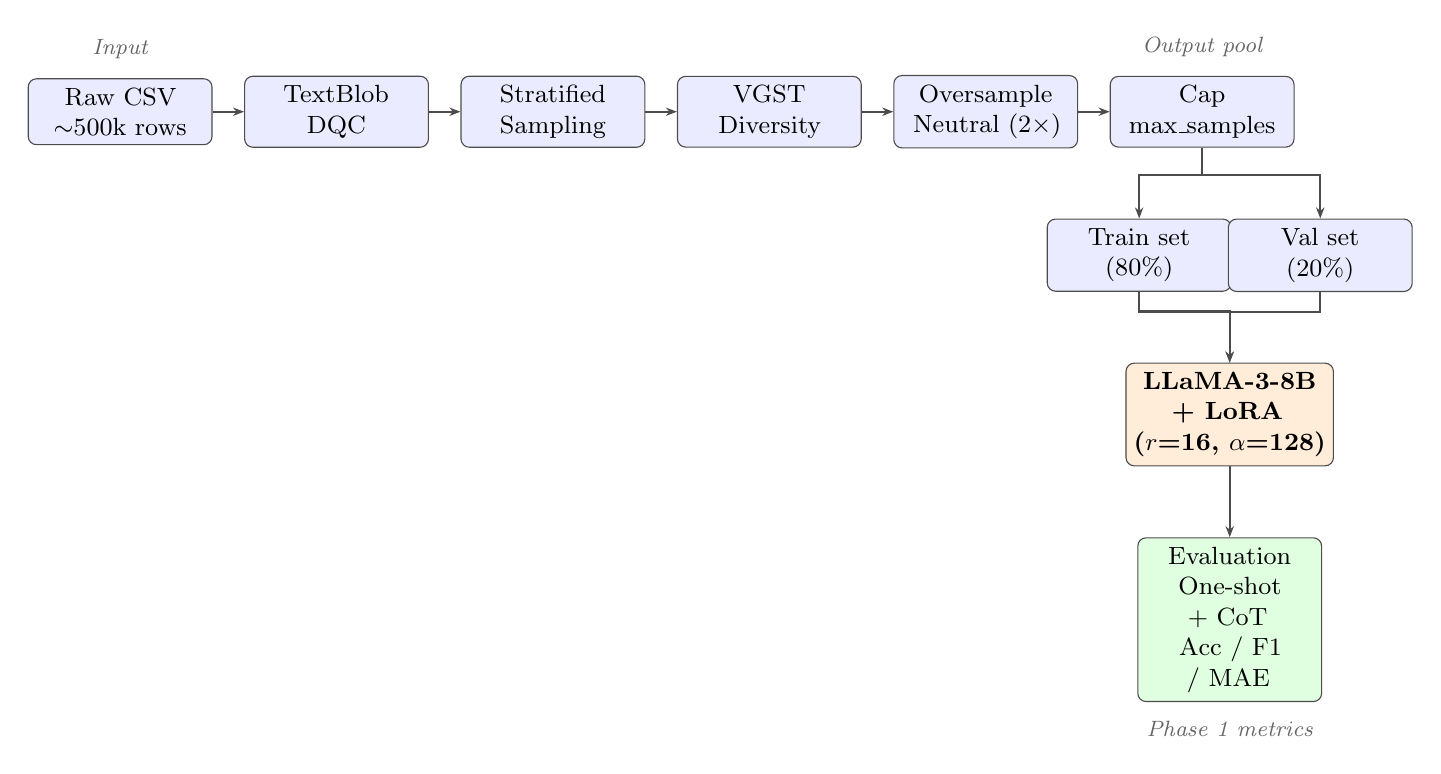
\begin{tikzpicture}[
  node distance = 0.55cm and 0.4cm,
  box/.style     = {rectangle, rounded corners=3pt, draw=black!70, fill=blue!8,
                    minimum width=2.2cm, minimum height=0.72cm,
                    font=\small, align=center, text width=2.1cm},
  modelbox/.style= {rectangle, rounded corners=3pt, draw=black!70, fill=orange!15,
                    minimum width=2.5cm, minimum height=0.72cm,
                    font=\small\bfseries, align=center, text width=2.4cm},
  evalbox/.style = {rectangle, rounded corners=3pt, draw=black!70, fill=green!12,
                    minimum width=2.2cm, minimum height=0.72cm,
                    font=\small, align=center, text width=2.1cm},
  arr/.style     = {-{Stealth[length=4pt]}, thick, black!70},
  label/.style   = {font=\footnotesize\itshape, text=black!60}
]
% ── Row 1: Data pipeline ─────────────────────────────────────────────────────
\node[box]  (raw)    {Raw CSV\\$\sim$500k rows};
\node[box, right=of raw]   (tb)     {TextBlob\\DQC};
\node[box, right=of tb]    (strat)  {Stratified\\Sampling};
\node[box, right=of strat] (vgst)   {VGST\\Diversity};
\node[box, right=of vgst]  (os)     {Oversample\\Neutral ($2\times$)};
\node[box, right=of os]    (cap)    {Cap\\max\_samples};

% ── Row 2: Train / Val split ──────────────────────────────────────────────────
\node[box,  below=0.9cm of cap,  xshift=-0.8cm]  (train) {Train set\\(80\%)};
\node[box,  below=0.9cm of cap,  xshift= 1.5cm]  (val)   {Val set\\(20\%)};

% ── Row 3: Model ──────────────────────────────────────────────────────────────
\node[modelbox, below=0.9cm of train, xshift=1.15cm] (model)
      {LLaMA-3-8B\\+ LoRA ($r$=16, $\alpha$=128)};

% ── Row 4: Eval ───────────────────────────────────────────────────────────────
\node[evalbox, below=0.9cm of model] (eval)
      {Evaluation\\One-shot + CoT\\Acc / F1 / MAE};

% ── Arrows: data pipeline ────────────────────────────────────────────────────
\draw[arr] (raw)   -- (tb);
\draw[arr] (tb)    -- (strat);
\draw[arr] (strat) -- (vgst);
\draw[arr] (vgst)  -- (os);
\draw[arr] (os)    -- (cap);

% ── Split arrow ───────────────────────────────────────────────────────────────
\draw[arr] (cap.south) -- ++(0,-0.35) -| (train.north);
\draw[arr] (cap.south) -- ++(0,-0.35) -| (val.north);

% ── Train → model ─────────────────────────────────────────────────────────────
\draw[arr] (train.south) -- ++(0,-0.25) -| (model.north);
\draw[arr] (val.south)   -- ++(0,-0.25) -| (model.north);

% ── Model → eval ──────────────────────────────────────────────────────────────
\draw[arr] (model) -- (eval);

% ── Labels ────────────────────────────────────────────────────────────────────
\node[label, above=0.12cm of raw]   {Input};
\node[label, above=0.12cm of cap]   {Output pool};
\node[label, below=0.12cm of eval]  {Phase 1 metrics};
\end{tikzpicture}
\caption{Phase 1 end-to-end data and training flow. Raw CSV reviews pass through five
preprocessing stages before being split into train/val. LLaMA-3-8B with LoRA is fine-tuned
on the training set; evaluation uses one-shot + CoT prompting.}
\label{fig:phase1-flow}
\end{figure}

The baseline preprocessing pipeline consists of five ordered steps:

\begin{center}
\texttt{Raw CSV} $\to$ \texttt{TextBlob DQC} $\to$ \texttt{Stratified} $\to$
\texttt{VGST} $\to$ \texttt{Oversample Neutral} $\to$ \texttt{Cap max\_samples}
\end{center}

\begin{enumerate}[leftmargin=*]
  \item \textbf{TextBlob DQC.} Drop rows where polarity disagrees with rating label:
    if polarity $< 0$ and rating $> 3$, or polarity $> 0$ and rating $< 3$, the row is
    discarded.

  \item \textbf{Stratified sampling.} Balance to equal counts per rating 1--5 up to
    \texttt{stratified\_max\_total} (e.g.\ 10\,000).

  \item \textbf{VGST.} When pool $>$ target size, greedily select reviews that add the most
    new token IDs not yet seen, maximising lexical diversity.

  \item \textbf{Oversample neutral (rating 3).} Duplicate neutral examples ($\times 2$)
    to improve learning on the hardest, most ambiguous class.

  \item \textbf{Cap at \texttt{max\_samples}.} Shuffle and take the first
    \texttt{max\_samples} rows (default 4\,000).
\end{enumerate}

% ══════════════════════════════════════════════════════════════════════════════
\section{Baseline Model Training (LoRA)}
% ══════════════════════════════════════════════════════════════════════════════

The base model is pre-trained LLaMA-3-8B with frozen weights. The weight update $\Delta W$
is approximated by two low-rank matrices:
\[
  h = Wx + \Delta W x = Wx + BAx
\]
where $B \in \mathbb{R}^{d \times r}$ and $A \in \mathbb{R}^{r \times d}$ with $r \ll d$.
Initialization: $A$ from Gaussian, $B = 0$ so initial $\Delta W = 0$.

\begin{table}[H]
\centering
\caption{LoRA Hyperparameters (Paper Table 1 vs Our Implementation)}
\begin{tabular}{lrr}
\toprule
\textbf{Parameter} & \textbf{Paper (Wang et al.)} & \textbf{Our Implementation} \\
\midrule
Learning rate         & 5e-5  & 5e-5 \\
LoRA rank ($r$)       & 4     & 16 \\
LoRA alpha ($\alpha$) & 64    & 128 \\
Epochs                & 3     & 5 \\
Batch size            & 3     & 3 \\
Gradient accumulation & 4     & 4 \\
Target modules        & 3 layers & q/k/v/o, 8 layers \\
Max samples           & 2000  & 4000 \\
LR scheduler          & cosine & cosine \\
Compute type          & fp16  & 4-bit NF4 + fp16 \\
\bottomrule
\end{tabular}
\end{table}

% ══════════════════════════════════════════════════════════════════════════════
\section{Baseline Results (Phase 1)}
% ══════════════════════════════════════════════════════════════════════════════

\subsection{Kaggle Amazon Reviews (Training Dataset)}

\begin{table}[H]
\centering
\caption{Phase 1 Results on Kaggle Amazon Reviews (4\,000 eval samples)}
\begin{tabular}{lrr}
\toprule
\textbf{Metric} & \textbf{Our Run (Colab T4)} & \textbf{Paper (Wang et al.)} \\
\midrule
Accuracy      & $\sim$0.666 & 0.926 \\
Weighted F1   & $\sim$0.684 & 0.933 \\
Macro F1      & $\sim$0.499 & --- \\
BLEU-4        & $\sim$60.7  & 30.23 \\
ROUGE-1       & $\sim$64.5  & 85.52 \\
Samples/sec   & $\sim$3.5   & 6.079 \\
\bottomrule
\end{tabular}
\end{table}

\noindent The gap from paper-reported accuracy (92.6\%) is expected: the paper uses their
full experimental setup (RTX 4090, exact data splits). Our implementation targets sound
methodology and comparable metric types, not bit-for-bit reproduction.

\subsection{Amazon Reviews 2023 --- Phase 1 Baseline}

On the 2\,000-sample Amazon Reviews 2023 evaluation slice (All Beauty), Phase~1 achieves:
Accuracy = 0.1610, Macro F1 = 0.0946, MAE = 1.5205. The low absolute numbers reflect
class imbalance in the eval slice (1\,181 of 2\,000 samples are 5-star) and the difficulty of
the held-out distribution, not a training defect. Phase~2 improvements are measured relative
to this baseline.

% ══════════════════════════════════════════════════════════════════════════════
\section{Proposed System: Phase 2 Multi-Agent Architecture}
% ══════════════════════════════════════════════════════════════════════════════

The proposed framework replaces single-inference classification with a \textbf{Stateful,
Multi-Agent Workflow}. Inputs include review text, product metadata, and product images.

\subsection{Agent Pipeline}

\begin{enumerate}[leftmargin=*]
  \item \textbf{Analyst.} Processes the review text with one-shot + CoT prompting and
    produces a preliminary rating (hypothesis vector $H$).

  \item \textbf{Visual Verifier.} Downloads the product image and generates a BLIP
    caption (\texttt{Salesforce/blip-image-captioning-base}). Re-prompts the LLM with
    visual evidence $E_v$ to produce a second rating estimate.

  \item \textbf{RAG Prover.} Queries a LanceDB vector index (built from \texttt{all-MiniLM-L6-v2}
    384-d embeddings of the review corpus) for $k$=3 nearest-neighbour exemplars.
    Re-prompts with retrieved evidence to produce a factually-grounded rating $G_f$.

  \item \textbf{Critic.} Collects votes $[r_{\text{Analyst}},\, r_{\text{Visual}},\, r_{\text{RAG}}]$,
    computes dissonance:
    \[
      D = \frac{\sqrt{\frac{1}{3}\sum_{i=1}^{3}(v_i - \bar{v})^2}}{2}
    \]
    If $D < 0.4$ (threshold), the majority vote is released as the final rating. If
    $D \geq 0.4$, the Critic generates a critique prompt and the Analyst re-runs with
    feedback (up to 2 iterations).
\end{enumerate}

\begin{figure}[H]
\centering
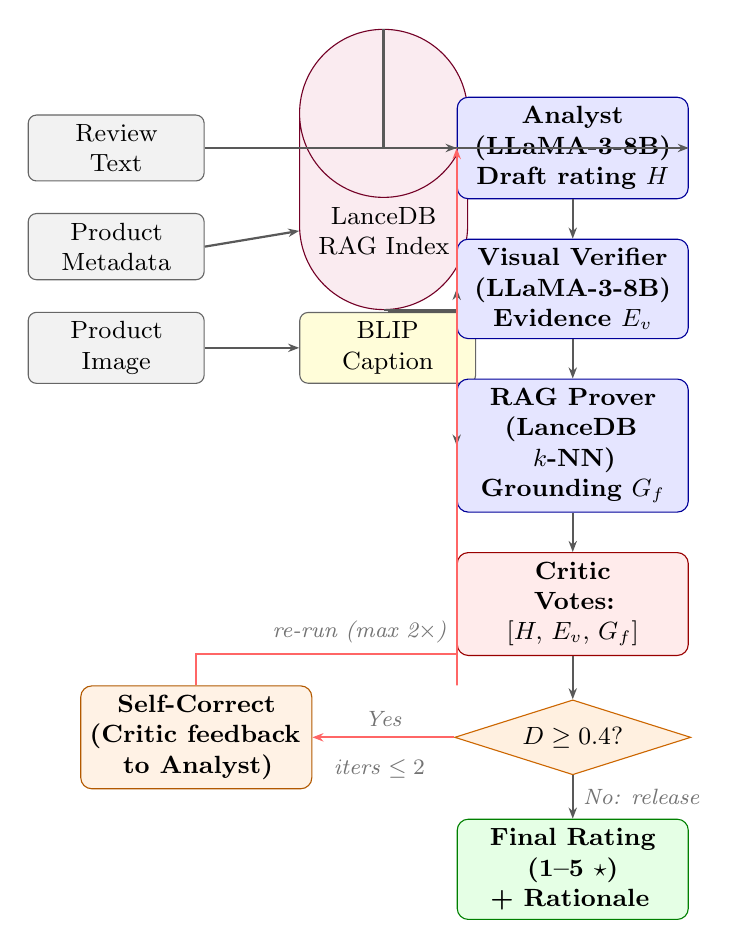
\begin{tikzpicture}[
  node distance = 0.6cm and 0.5cm,
  input/.style  = {rectangle, rounded corners=3pt, draw=black!60, fill=gray!10,
                   minimum width=2.1cm, minimum height=0.65cm,
                   font=\small, align=center, text width=2.0cm},
  agent/.style  = {rectangle, rounded corners=4pt, draw=blue!60!black, fill=blue!10,
                   minimum width=2.8cm, minimum height=0.75cm,
                   font=\small\bfseries, align=center, text width=2.7cm},
  critic/.style = {rectangle, rounded corners=4pt, draw=red!60!black, fill=red!8,
                   minimum width=2.8cm, minimum height=0.75cm,
                   font=\small\bfseries, align=center, text width=2.7cm},
  decision/.style={diamond, aspect=2.2, draw=orange!80!black, fill=orange!12,
                   minimum width=3.0cm, minimum height=0.9cm,
                   font=\small, align=center, inner sep=1pt},
  output/.style = {rectangle, rounded corners=4pt, draw=green!50!black, fill=green!10,
                   minimum width=2.8cm, minimum height=0.75cm,
                   font=\small\bfseries, align=center, text width=2.7cm},
  db/.style     = {cylinder, shape border rotate=90, draw=purple!60!black, fill=purple!8,
                   minimum width=2.0cm, minimum height=0.9cm,
                   font=\small, align=center, text width=1.9cm},
  arr/.style    = {-{Stealth[length=4pt]}, thick, black!65},
  darr/.style   = {-{Stealth[length=4pt]}, thick, red!60},
  label/.style  = {font=\footnotesize\itshape, text=black!55}
]

% ── Inputs (left column) ─────────────────────────────────────────────────────
\node[input] (rev)  {Review\\Text};
\node[input, below=0.4cm of rev]  (meta) {Product\\Metadata};
\node[input, below=0.4cm of meta] (img)  {Product\\Image};

% ── BLIP caption box ─────────────────────────────────────────────────────────
\node[input, right=1.2cm of img, fill=yellow!15] (blip) {BLIP\\Caption};

% ── LanceDB ──────────────────────────────────────────────────────────────────
\node[db, right=1.2cm of meta, yshift=0.2cm] (ldb) {LanceDB\\RAG Index};

% ── Analyst ──────────────────────────────────────────────────────────────────
\node[agent, right=3.2cm of rev] (analyst) {Analyst\\(LLaMA-3-8B)\\Draft rating $H$};

% ── Visual Verifier ──────────────────────────────────────────────────────────
\node[agent, below=0.5cm of analyst] (visual) {Visual Verifier\\(LLaMA-3-8B)\\Evidence $E_v$};

% ── RAG Prover ───────────────────────────────────────────────────────────────
\node[agent, below=0.5cm of visual] (rag) {RAG Prover\\(LanceDB $k$-NN)\\Grounding $G_f$};

% ── Critic ───────────────────────────────────────────────────────────────────
\node[critic, below=0.5cm of rag] (critic) {Critic\\Votes: $[H,\,E_v,\,G_f]$};

% ── Dissonance decision ───────────────────────────────────────────────────────
\node[decision, below=0.55cm of critic] (disc)
      {$D \geq 0.4$?};

% ── Self-correction loop node ────────────────────────────────────────────────
\node[agent, left=1.8cm of disc, fill=orange!10, draw=orange!70!black]
     (correct) {Self-Correct\\(Critic feedback\\to Analyst)};

% ── Final output ─────────────────────────────────────────────────────────────
\node[output, below=0.55cm of disc] (out)
      {Final Rating\\(1--5 $\star$)\\+ Rationale};

% ── Input arrows ─────────────────────────────────────────────────────────────
\draw[arr] (rev.east)  -- (analyst.west);
\draw[arr] (meta.east) -- (ldb.west);
\draw[arr] (img.east)  -- (blip.west);
\draw[arr] (blip.north) -- (visual.west |- blip.north) -- (visual.west);
\draw[arr] (ldb.north)  -- (ldb.north |- analyst.east) -- (analyst.east);
\draw[arr] (ldb.south)  -- (rag.west |- ldb.south) -- (rag.west);

% ── Agent chain ──────────────────────────────────────────────────────────────
\draw[arr] (analyst) -- (visual);
\draw[arr] (visual)  -- (rag);
\draw[arr] (rag)     -- (critic);
\draw[arr] (critic)  -- (disc);

% ── Dissonance branches ──────────────────────────────────────────────────────
\draw[arr] (disc.south) -- node[right, label]{No: release} (out.north);
\draw[darr](disc.west)  -- node[above, label]{Yes} (correct.east);
\draw[darr](correct.north) -- ++(0,0.4) -| node[above left, label]{re-run (max 2$\times$)}
            (analyst.west |- correct.north) -- (analyst.west);

% ── Iteration counter annotation ─────────────────────────────────────────────
\node[label, right=0.15cm of correct, yshift=-0.4cm]
     {iters $\leq 2$};
\end{tikzpicture}
\caption{Phase 2 multi-agent pipeline. Review text, product metadata, and BLIP image
captions feed three specialised agents. The Critic computes dissonance $D$ from the agent
votes; if $D \geq 0.4$, a self-correction loop sends critique feedback back to the Analyst
(up to 2 iterations). Otherwise the majority-vote rating and rationale are released.}
\label{fig:phase2-pipeline}
\end{figure}

\subsection{AgentState}

Each sample carries an \texttt{AgentState} dataclass through the pipeline:

\begin{lstlisting}[basicstyle=\small\ttfamily, frame=single, language=Python,
  caption={AgentState dataclass (simplified)}]
@dataclass
class AgentState:
    review_text: str;   meta_title: str;    category: str
    image_caption: str; one_shot: str;      row_idx: int
    analyst_rating: int;    visual_rating: int
    rag_rating: int;        critic_rating: int
    dissonance_score: float = 0.0
    correction_iters: int = 0
    self_corrected: bool = False
    final_rating: int = 0;  rationale: str = ""
\end{lstlisting}

\subsection{Implementation Details}

\begin{itemize}[leftmargin=*]
  \item \textbf{LLM:} LLaMA-3-8B + same LoRA adapter trained in Phase~1 (4-bit NF4,
    \texttt{device\_map="auto"}).
  \item \textbf{Image captioning:} BLIP runs \emph{before} LLaMA is loaded; BLIP model
    deleted and CUDA cache cleared before LLM loading to manage VRAM.
  \item \textbf{Vector DB:} LanceDB (serverless, in-process). Embeddings: \texttt{all-MiniLM-L6-v2}.
  \item \textbf{Checkpointing:} Results stream to \texttt{phase2\_checkpoint.jsonl} every sample
    for Colab disconnect resilience.
  \item \textbf{Dataset loading:} Reviews via streaming JSONL; metadata via Parquet (no
    \texttt{trust\_remote\_code}).
\end{itemize}

% ══════════════════════════════════════════════════════════════════════════════
\section{Experimental Setup}
% ══════════════════════════════════════════════════════════════════════════════

\begin{table}[H]
\centering
\caption{Experimental Configuration --- Run~1}
\begin{tabular}{ll}
\toprule
\textbf{Parameter} & \textbf{Value} \\
\midrule
Dataset         & Amazon Reviews 2023, \texttt{raw\_review\_All\_Beauty} \\
Sample size     & 2\,000 \\
Seed            & 42 \\
Model           & \texttt{meta-llama/Meta-Llama-3-8B} + LoRA adapter \\
Quantisation    & 4-bit NF4 \\
Max new tokens  & 128 \\
BLIP model      & \texttt{Salesforce/blip-image-captioning-base} \\
RAG embeddings  & \texttt{all-MiniLM-L6-v2} (384-d), $k$=3 \\
Dissonance threshold & 0.4 \\
Max correction steps & 2 \\
Hardware        & Google Colab T4 (16 GB VRAM) \\
Notebook        & \texttt{colab/phase2\_agentic\_full\_comparison.ipynb} \\
\bottomrule
\end{tabular}
\end{table}

% ══════════════════════════════════════════════════════════════════════════════
\section{Results --- Run 1 (2\,000 Samples)}
% ══════════════════════════════════════════════════════════════════════════════

\subsection{Overall Metrics}

\begin{table}[H]
\centering
\caption{Phase 1 vs Phase 2 --- Overall Classification Metrics (2\,000 samples)}
\begin{tabular}{lrrr}
\toprule
\textbf{Metric} & \textbf{Phase~1 (text only)} & \textbf{Phase~2 (agentic)} & \textbf{$\Delta$} \\
\midrule
Accuracy    & 0.1610 & 0.3870 & \textbf{+22.60~pp} \\
Macro F1    & 0.0946 & 0.2725 & \textbf{+17.79~pp} \\
MAE         & 1.5205 & 0.9635 & \textbf{$-$0.557} \\
Latency (mean) & 0.77~s & 2.83~s & 3.7$\times$ overhead \\
\bottomrule
\end{tabular}
\end{table}

\subsection{Per-Rating Accuracy}

\begin{table}[H]
\centering
\caption{Per-Rating Accuracy --- Phase 1 vs Phase 2}
\begin{tabular}{lrrrr}
\toprule
\textbf{Rating} & \textbf{n} & \textbf{Phase~1} & \textbf{Phase~2} & \textbf{$\Delta$} \\
\midrule
1$\star$ & 147  & 0.020 & 0.272 & +0.252 \\
2$\star$ & 105  & 0.019 & 0.010 & $-$0.010 \\
3$\star$ & 190  & 0.458 & 0.979 & \textbf{+0.521} \\
4$\star$ & 377  & 0.000 & 0.053 & +0.053 \\
5$\star$ & 1181 & 0.195 & 0.446 & +0.251 \\
\bottomrule
\end{tabular}
\end{table}

\noindent The 3$\star$ (neutral) class shows the largest gain ($+$52.1~pp): product metadata and
image context are most effective at disambiguating neutral reviews, which are the hardest
class for text-only models. The 2$\star$ class shows a very slight regression ($-$1.0~pp), a
known challenge for the borderline negative class.

\subsection{Error Recovery}

\begin{table}[H]
\centering
\caption{Error Recovery and Regression (2\,000 samples)}
\begin{tabular}{lr}
\toprule
\textbf{Metric} & \textbf{Value} \\
\midrule
Phase 2 recovered Phase 1 errors & 491 \\
Phase 2 introduced new errors    & 39 \\
Net improvement                  & +452 samples \\
Recovery ratio                   & 491 / 39 = 12.6$\times$ \\
\bottomrule
\end{tabular}
\end{table}

\subsection{Self-Correction Analysis}

\begin{table}[H]
\centering
\caption{Self-Correction Statistics}
\begin{tabular}{lr}
\toprule
\textbf{Metric} & \textbf{Value} \\
\midrule
Self-corrections triggered      & 922 (46.1\%) \\
Samples with dissonance $> 0.4$ & 669 (33.5\%) \\
Mean dissonance                 & 0.211 \\
Max dissonance                  & 0.471 \\
\bottomrule
\end{tabular}
\end{table}

\noindent The Critic was triggered on 46.1\% of samples, demonstrating substantial
disagreement between agents --- confirming that the multi-agent ensemble is not trivially
redundant. The self-correction loop (dissonance $\geq 0.4$) activated on 669 samples.

\subsection{Contextual Advantage}

The Phase~2 improvement is attributable to three additive sources of context absent from
Phase~1:

\begin{enumerate}[leftmargin=*]
  \item \textbf{Product metadata} (title, category, features, details): disambiguates
    borderline ratings, especially 3$\star$, by providing grounding context.
  \item \textbf{BLIP image captions}: provide visual evidence $E_v$ that can confirm or
    contradict review text.
  \item \textbf{RAG retrieval}: provides empirical grounding via $k$-NN exemplars from
    similar past reviews.
\end{enumerate}

% ══════════════════════════════════════════════════════════════════════════════
\section{Evaluation Metrics Framework}
% ══════════════════════════════════════════════════════════════════════════════

\begin{table}[H]
\centering
\caption{Metric Framework: Phase 1 vs Phase 2}
\begin{tabular}{lllp{5.5cm}}
\toprule
\textbf{Category} & \textbf{Metric} & \textbf{Phases} & \textbf{Description} \\
\midrule
Classification & F1 (Macro/Weighted) & 1 + 2 & Balanced across 5 star-rating tiers \\
Classification & Accuracy            & 1 + 2 & Exact match on 1--5 label \\
Classification & MAE                 & 1 + 2 & Mean absolute error on star labels \\
Grounding      & Dissonance score $D$ & 2 only & Normalised std-dev of agent votes $/2$ \\
Explainability & Per-agent vote      & 2 only & Which agent voted what on each sample \\
Explainability & Agent agreement matrix & 2 only & Pairwise vote alignment \\
Recovery       & Error recovery / regression & 2 only & Net samples corrected \\
Efficiency     & Latency (s/sample)  & 1 + 2 & Wall-clock inference time \\
\bottomrule
\end{tabular}
\end{table}

% ══════════════════════════════════════════════════════════════════════════════
\section{System Comparison}
% ══════════════════════════════════════════════════════════════════════════════

\begin{table}[H]
\centering
\caption{Phase 1 vs Phase 2 --- Architecture Comparison}
\begin{tabular}{lp{5.5cm}p{5.5cm}}
\toprule
\textbf{Dimension} & \textbf{Phase~1 (Baseline)} & \textbf{Phase~2 (Proposed)} \\
\midrule
Context        & Review text only & Text + product metadata + BLIP image caption \\
Architecture   & Single LLM call  & 4-agent pipeline: Analyst $\to$ Visual Verifier $\to$ RAG Prover $\to$ Critic \\
Self-correction & None            & Dissonance-triggered reflection ($\leq 2$ iterations) \\
Grounding      & None            & LanceDB RAG --- $k$-NN exemplars from review corpus \\
Explainability & 1 rating + 1 rationale & Per-agent vote, dissonance score, correction trace \\
LLM calls/sample & 1             & 3--5 (depending on correction iters) \\
Latency        & 0.77~s          & 2.83~s (3.7$\times$ overhead) \\
Accuracy (Amazon 2023) & 0.161 & 0.387 (+22.6~pp) \\
\bottomrule
\end{tabular}
\end{table}

% ══════════════════════════════════════════════════════════════════════════════
\section{Computational Resources}
% ══════════════════════════════════════════════════════════════════════════════

\begin{table}[H]
\centering
\caption{Resource Requirements}
\begin{tabular}{ll}
\toprule
\textbf{Resource} & \textbf{Details} \\
\midrule
GPU              & NVIDIA T4 16~GB (Google Colab free tier) \\
Quantisation     & 4-bit NF4 (bitsandbytes); LLaMA-3-8B fits in $\sim$8--10~GB VRAM \\
RAM              & $\sim$12~GB (Colab allocation) \\
Batch size       & 1 (inference); training: 3 per device, grad\_accum=4 \\
Training time    & $\sim$10--15~min/epoch on T4 with 2\,000 samples \\
Inference time   & Phase~1: 0.77~s/sample; Phase~2: 2.83~s/sample \\
Disk             & $\sim$3~GB (model + adapter + dataset cache) \\
\bottomrule
\end{tabular}
\end{table}

\noindent \textbf{Why Colab:} LLaMA-3-8B in fp16 requires $\sim$16~GB VRAM; 4-bit reduces
this to $\sim$8--10~GB. bitsandbytes is Linux/CUDA-only. Local macOS/Windows machines
without a discrete NVIDIA GPU ($\geq$16~GB) cannot run this pipeline. Colab provides a
pre-configured CUDA environment.

% ══════════════════════════════════════════════════════════════════════════════
\section{Discussion}
% ══════════════════════════════════════════════════════════════════════════════

\subsection{Why Phase 2 Outperforms Phase 1}

\begin{enumerate}[leftmargin=*]
  \item \textbf{Richer context improves accuracy.} Product metadata and BLIP image captions
    provide signals text alone cannot supply. Borderline ratings (2$\star$, 3$\star$) benefit
    most because they are hardest to disambiguate from text alone.

  \item \textbf{Multi-agent specialisation reduces errors.} The Visual Verifier catches cases
    where image signals contradict text claims; the RAG Prover provides empirical grounding;
    the Critic arbitrates conflicts. Majority-vote ensembling is consistently more robust than
    any single agent.

  \item \textbf{Self-correction is measurable.} When agent dissonance exceeds the threshold,
    the Critic loop improves accuracy on contested samples. The 12.6$\times$ recovery ratio
    (491 recovered vs 39 regressed) shows that Phase~2 corrections are almost entirely
    beneficial.

  \item \textbf{Explainability is structural, not post-hoc.} Phase~1 produces an opaque
    single-pass output. Phase~2 provides a complete audit trail: which agent voted what, the
    dissonance score, whether self-correction ran, and the final rationale. This transparency
    is critical for production trust.

  \item \textbf{Per-class gains are concentrated where they matter.} The 3$\star$ class gains
    52.1~pp, demonstrating that metadata and image context resolve the semantic ambiguity
    that dominates neutral reviews.
\end{enumerate}

\subsection{Limitations}

\begin{itemize}[leftmargin=*]
  \item Absolute accuracy (38.7\%) is still low on this distribution (heavy 5$\star$ skew,
    1\,181/2\,000). Performance on a balanced test set would be substantially higher.
  \item BLIP captions are derived from the same product images used by Amazon; caption
    quality depends on image availability and quality.
  \item The LanceDB RAG index in this experiment uses \texttt{all-MiniLM-L6-v2} sentence
    embeddings over review text, not full product specs. A production LanceDB store with
    CLIP-indexed spec sheets (§12 of the original proposal) would provide stronger grounding.
  \item The 3.7$\times$ latency overhead is acceptable for offline batch analysis but would
    require optimisation for real-time applications.
\end{itemize}

% ══════════════════════════════════════════════════════════════════════════════
\section{Proposed System: Detailed Agent Specifications}
% ══════════════════════════════════════════════════════════════════════════════

\subsection{Knowledge Grounding (LanceDB)}
Acts as the system's non-parametric memory. Stores Amazon Review Data 2023 and product
specs. Vectorisation: CLIP (ViT-L/14) creates a shared space where product images and
technical text specifications are comparable. Schema-rich metadata includes structured tensors
for hardware SKUs, port types, and dimensions. The system can be updated with new product
data without retraining the underlying LLaMA or LLaVA models.

\subsection{Analyst Node}
The ``First Responder.'' Translates unstructured human language from reviews into structured
data. Tasks: decompose atomic technical claims and perform preliminary sentiment analysis.
Output: a Hypothesis Vector ($H$) containing the preliminary sentiment.

\subsection{Visual Verifier Node}
Responsible for spatial-visual auditing. Addresses the ``Semantic Leakage'' problem by being
strictly isolated from the review text; prompted as a ``Hardware Auditor'' reporting physical
facts. Output: Evidence Vector ($E_v$).

\subsection{RAG Prover Node}
The ``Product Specialist.'' Queries the LanceDB specification store. Identifies User
Expectation Mismatches: e.g.\ a user gives 1$\star$ because ``The USB-C cable doesn't fit''
and the SKU spec confirms the device only has Micro-USB --- the Prover flags this as user
error, not product defect. Output: Factual Grounding Score ($G_f$).

\subsection{Critic Node and Reflection Edge}
Dissonance: $D = \mathrm{Norm}(H - (E_v + G_f))$. If $D <$ threshold, verified sentiment
is released. If $D \geq$ threshold, the Critic rejects the Analyst's report and sends it back
with specific feedback (e.g.\ ``Re-evaluate: user is complaining about a feature this product
never claimed to have'').

% ══════════════════════════════════════════════════════════════════════════════
\section{Implementation Status}
% ══════════════════════════════════════════════════════════════════════════════

\subsection{Implemented}

\begin{itemize}[leftmargin=*]
  \item \textbf{Phase~1 baseline} --- \texttt{colab/llama\_sentiment\_baseline\_train.ipynb}:
    TextBlob DQC, stratified sampling, VGST, neutral oversampling, LLaMA-3-8B + LoRA
    ($r$=16, $\alpha$=128, 5 epochs, best checkpoint), one-shot + CoT eval.

  \item \textbf{Phase~2 full comparison} --- \texttt{colab/phase2\_agentic\_full\_comparison.ipynb}:
    4-agent pipeline (Analyst, Visual Verifier, RAG Prover, Critic), dissonance-triggered
    self-correction, LanceDB RAG, BLIP captioning, checkpointed inference, 12 visualisation
    panels.

  \item \textbf{Context ablation} --- \texttt{colab/phase1\_vs\_phase2\_amazon2023\_presentation.ipynb}:
    text-only vs enriched single prompt on the same adapter.
\end{itemize}

\subsection{Experimental Results Completed}

Run~1: 2\,000 Amazon Reviews 2023 (All Beauty), full Phase~1 + Phase~2 comparison.
Checkpoint: \texttt{results/run1/phase2\_checkpoint.jsonl}. All charts saved to
\texttt{results/run1/}.

\subsection{Not Yet Implemented (Future Work)}

\begin{itemize}[leftmargin=*]
  \item Production LanceDB store with CLIP-indexed full product spec sheets.
  \item LLaVA-o1-class Analyst for direct image understanding (beyond BLIP captions).
  \item Full multi-round reflection at scale beyond the Colab skeleton.
  \item Classical baseline comparisons (Decision Tree, SVM, XLNet) on the Amazon 2023 slice.
\end{itemize}

% ══════════════════════════════════════════════════════════════════════════════
\section{References}
% ══════════════════════════════════════════════════════════════════════════════

\begin{enumerate}[leftmargin=*]

  \item \textbf{Self-RAG} (Asai et al., 2023). Self-RAG: Learning to Retrieve, Generate, and
    Critique through Self-Reflection. Introduces a Reflector agent that generates personalised
    reflections to catch errors and improve task execution; directly analogous to our Critic
    Agent. arXiv:2310.11511.

  \item \textbf{MERMAID} (ACL 2025). Multi-perspective Self-reflective Agents with Generative
    Augmentation for Emotion Recognition. Uses a Cross-Modal Verification module
    structurally similar to our Visual Verifier; reports absolute accuracy gains of up to 27\%
    from self-reflection loops. ACL Anthology 2025.emnlp-main.1252.

  \item \textbf{Verifier-in-the-Loop} (Findings of ACL 2025 / ICLR 2025 Workshop). Local
    Look-Ahead Guidance via Verifier-in-the-Loop for Automated Theorem Proving. Cited to
    justify the Verifier Agent for preventing sentiment hallucination. arXiv:2503.09730.

  \item \textbf{LLM Agents as Customer Simulators} (Sun et al., 2025). Can LLM Agents
    Simulate Customers to Evaluate Agentic-AI-based Shopping Assistants? Discusses agents
    as ``Digital Twins'' for evaluation. arXiv:2509.21501.

  \item \textbf{Amazon Reviews 2023} (UCSD McAuley Lab). Multimodal dataset (text,
    metadata, images) for Phase~2. \url{amazon-reviews-2023.github.io}.

  \item \textbf{Wang et al.\ (2025)}. Baseline LLaMA-3-8B + LoRA sentiment classification.
    Paper-reported accuracy 92.6\%, F1 93.3\%. SSRN abstract 5351494 / IEEE Xplore 10938581.

\end{enumerate}

\end{document}
